% =====================================================================
%  CDT503 Final Project Report —— IEEEtran 会议格式（4–6 页）
%  把 <...> 占位符替换成你们的数据；图放在 report/fig/ 下。
%  编译：pdflatex -> pdflatex（或直接用 Overleaf / TeXPage）
% =====================================================================
\documentclass[conference]{IEEEtran}
\IEEEoverridecommandlockouts

\usepackage{cite}
\usepackage{amsmath,amssymb,amsfonts}
\usepackage{graphicx}
\usepackage{textcomp}
\usepackage{xcolor}
\usepackage{booktabs}
\usepackage[hidelinks]{hyperref}

\begin{document}

\title{Credit Card Fraud Detection under Extreme Class Imbalance: \\
 A Class-Imbalance-Aware Deep Learning Prototype}

\author{
\IEEEauthorblockN{Feng Hongyuan, Zheng Xuan, Huang Guanrong}
\IEEEauthorblockA{\textit{CDT503 Control Systems and AI} \\
\textit{Lingnan University}\\
Hong Kong SAR, China \\
\{<email1>, <email2>, <email3>\}}
}

\maketitle

\begin{abstract}
Credit card fraud detection is a severely imbalanced classification problem:
only 0.17\% of transactions in the public benchmark are fraudulent, so a
trivial ``always normal'' classifier already reaches 99.83\% accuracy while
catching nothing. We build an end-to-end prototype that addresses this
imbalance explicitly. We compare four resampling and re-weighting strategies
(class weighting, weighted sampling, SMOTE, and random oversampling) on top of
three neural architectures, with a gradient-boosted tree as a reference.
Instead of the default 0.5 threshold, we select the decision threshold on a
validation set under an explicit cost model in which a missed fraud costs
20 times more than a false alarm, and we show that the resulting threshold
matches the Bayes-optimal value $c_{FP}/(c_{FN}+c_{FP})\approx0.048$. The best
model (MLP with SMOTE) reaches an AUC-PR of 0.8030 and a recall of 0.831 at a
cost of 289. Two findings are worth emphasising. Resampling raises AUC-PR by
roughly eight points over no handling, whereas class weighting raises it by
nothing and inflates the cost at the default threshold from 313 to 1192 by
destroying probability calibration. And the $F_1$-optimal threshold is a poor
proxy for the cost-optimal one: on three of nine configurations it is worse
than leaving the threshold at 0.5. The model is deployed as an interactive web
application that scores uploaded transaction batches.
\end{abstract}

\begin{IEEEkeywords}
fraud detection, class imbalance, cost-sensitive learning, threshold tuning,
AUC-PR, Gradio
\end{IEEEkeywords}

% ---------------------------------------------------------------- I
\section{Introduction and Problem Setup}
\label{sec:intro}

\IEEEPARstart{C}{ard-not-present} fraud causes losses of tens of billions of
US dollars annually. Rule-based systems are cheap to deploy but require
constant manual maintenance and degrade as fraudsters adapt, which motivates
learning-based detectors.

The central difficulty is not model capacity but data statistics: the public
benchmark contains 284{,}807 transactions of which only 492 (0.172\%) are
fraudulent, an imbalance ratio of roughly 1:579; after de-duplication 473
frauds remain out of 283{,}726 rows. Under this regime accuracy is
uninformative---predicting ``normal'' for every sample yields 99.83\%---and
even AUC-ROC is optimistic, because the large negative class keeps the
false-positive rate low for almost any threshold.

Our contributions are:
\begin{itemize}
  \item a reproducible pipeline covering de-duplication, leakage-free scaling,
        stratified splitting, and evaluation;
  \item a controlled comparison of four imbalance strategies across three
        neural architectures and one tree-based reference, which shows that
        \emph{resampling} improves ranking while \emph{re-weighting} does not,
        and that re-weighting additionally destroys calibration;
  \item a cost-sensitive threshold selection procedure whose empirical
        optimum reproduces the Bayes threshold
        $c_{FP}/(c_{FN}+c_{FP})$, together with evidence that the
        $F_1$-optimal threshold is often worse than the default;
  \item an interactive deployment that scores transaction batches in the
        browser.
\end{itemize}

\begin{figure}[t]
  \centering
  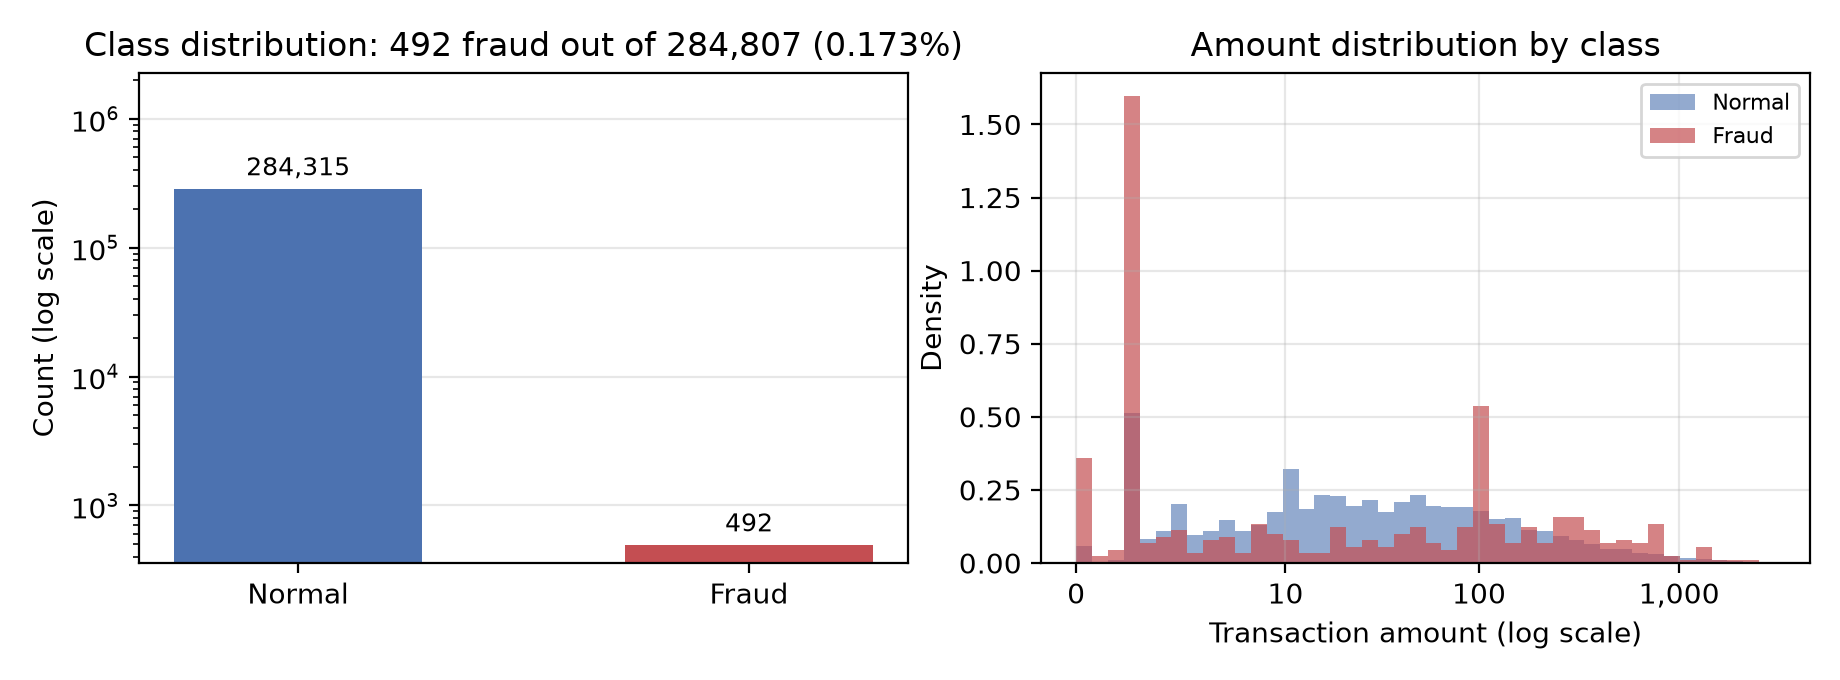
\includegraphics[width=\columnwidth]{fig/class_dist.png}
  \caption{Class distribution on a logarithmic scale. The minority class is
  0.172\% of the data, which makes accuracy meaningless.}
  \label{fig:dist}
\end{figure}

% ---------------------------------------------------------------- II
\section{Methodology and Architecture}
\label{sec:method}

\subsection{Pipeline}
Figure~\ref{fig:pipeline} summarises the system. Raw transactions are
de-duplicated and imputed, then split in a stratified 70/15/15 manner so that
the validation and test sets always contain fraud cases. The scaler is fitted
on the training split only; fitting it on the full data would leak test
statistics into training. Resampling is likewise applied to the training split
exclusively.

\begin{figure}[t]
  \centering
  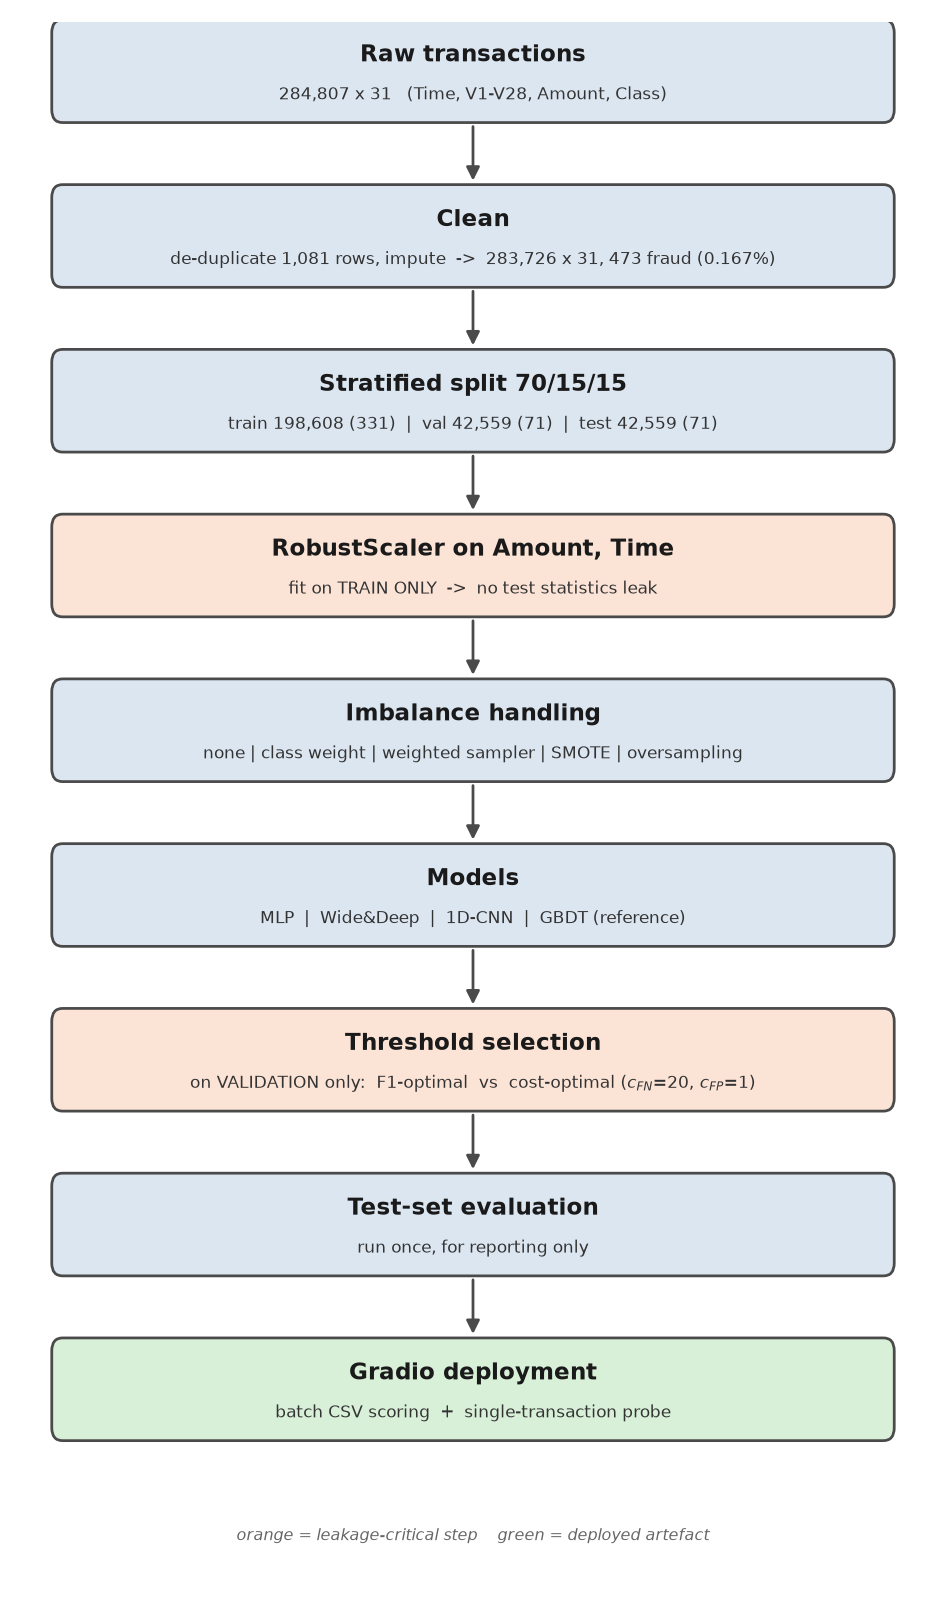
\includegraphics[width=\columnwidth]{fig/pipeline.png}
  \caption{System pipeline. The two leakage-critical steps are highlighted: the
  scaler is fitted on the training split only, and the decision threshold is
  selected on the validation split only. The test split is scored once, for
  reporting.}
  \label{fig:pipeline}
\end{figure}

\subsection{Class Imbalance}
Let $n^{+}$ and $n^{-}$ denote the numbers of fraudulent and normal training
transactions. The weighted binary cross-entropy is
\begin{equation}
  \mathcal{L} = -\frac{1}{N}\sum_{i=1}^{N}
  \Big[\, w\, y_i \log p_i + (1-y_i)\log(1-p_i) \Big],
  \qquad w = \frac{n^{-}}{n^{+}} \approx 579,
  \label{eq:wbce}
\end{equation}
which makes the two classes contribute equally to the gradient.

We compare this against three alternatives: (i) \emph{weighted sampling},
which draws mini-batches with class-balanced probability; (ii) \emph{SMOTE},
which synthesises minority points by interpolating between a sample and one of
its $k{=}5$ nearest minority neighbours,
$\tilde{x} = x_i + \lambda (x_j - x_i)$, $\lambda \sim U(0,1)$;
and (iii) \emph{random oversampling}, which duplicates minority points and
serves as a control for SMOTE.

\subsection{Architectures}
We evaluate three neural models: a three-layer MLP
($30\!\to\!128\!\to\!64\!\to\!32\!\to\!1$, BatchNorm and dropout $0.3$);
a Wide\,\&\,Deep model that sums a linear path with a two-layer nonlinear path;
and a 1D-CNN that treats the 30 features as a sequence. A histogram gradient
boosting classifier is included as a non-neural reference, since tree ensembles
are known to be strong on tabular data.

\subsection{Cost-Sensitive Threshold Selection}
A probability of 0.5 is meaningless after re-weighting, because the loss in
\eqref{eq:wbce} shifts the predicted probabilities upwards. We therefore treat
the threshold $\tau$ as a decision variable and choose it on the validation
set, never on the test set. Under the cost model
\begin{equation}
  \mathrm{Cost}(\tau) = c_{FN}\cdot \mathrm{FN}(\tau) + c_{FP}\cdot \mathrm{FP}(\tau),
  \qquad c_{FN}=20,\; c_{FP}=1,
  \label{eq:cost}
\end{equation}
the Bayes-optimal decision rule is to flag a transaction whenever
\begin{equation}
  p(y{=}1\mid x) \;>\; \tau^{*} = \frac{c_{FP}}{c_{FN}+c_{FP}} = \frac{1}{21} \approx 0.048 .
  \label{eq:taustar}
\end{equation}
This closed form is useful for two reasons. First, it shows that the optimal
threshold is set by the cost ratio alone and has nothing to do with 0.5.
Second, it gives a sanity check on the empirical procedure: the threshold we
select by minimising \eqref{eq:cost} on the validation set is
$\tau=0.049$, which matches $\tau^{*}$ to within one grid step.
We report three operating points---$\tau{=}0.5$, $\tau_{F1}$ (maximises
$F_1$), and $\tau_{cost}$ (minimises \eqref{eq:cost})---to show that $F_1$
and the business objective disagree.

\begin{table}[t]
\caption{Training Configuration}
\label{tab:config}
\centering
\begin{tabular}{ll}
\toprule
Item & Value \\
\midrule
Features        & V1--V28, Amount, Time (30) \\
Scaling         & RobustScaler on Amount/Time, fit on train \\
Split           & stratified 70/15/15 \\
Optimizer       & AdamW ($\beta_1{=}0.9$, $\beta_2{=}0.999$) \\
Learning rate   & $1\times10^{-3}$, cosine annealing \\
Weight decay    & $1\times10^{-4}$ \\
Batch size      & 1024 \\
Epochs          & 30 (early stopping, patience 8) \\
Model selection & validation AUC-PR \\
Hardware        & Apple M4 (MPS), 16\,GB \\
\bottomrule
\end{tabular}
\end{table}

% ---------------------------------------------------------------- III
\section{Implementation and Results}
\label{sec:results}

\subsection{Experimental Setup}
The raw dataset contains 284{,}807 transactions with 30 features. Removing
1{,}081 duplicate rows leaves 283{,}726 transactions, of which 473 are
fraudulent (0.167\%, an imbalance ratio of 1:600). Note that de-duplication
removes 19 fraud cases, which suggests that duplicates are not class-neutral
and that dropping them is not a formality. A stratified 70/15/15 split yields
198{,}608 training, 42{,}559 validation and 42{,}559 test transactions; the
validation and test sets contain 71 fraud cases each. All experiments use
seed 42.

\subsection{Main Results}
Table~\ref{tab:results} reports the nine configurations. Four observations
matter.

First, the unweighted baseline does \emph{not} collapse. Its AUC-PR is 0.7196
and its recall at the tuned threshold is 0.789, which is within one standard
error of the best model. The common claim that a model trained on 0.17\%
positive data learns nothing is false once the decision threshold is tuned:
the network still ranks transactions well, and most of the apparent failure of
an untuned baseline is a threshold artefact, not a representation failure.

Second, resampling improves ranking, whereas re-weighting does not. SMOTE
reaches an AUC-PR of 0.8030, random oversampling 0.7946 and weighted sampling
0.7887, against 0.7196 for no handling and 0.7047 for class weighting---an
absolute gain of roughly eight points. The mechanism is sample efficiency
rather than loss shaping: with 331 positives in 198{,}608 training rows, a
weighted model still sees only 331 positive examples per epoch, while
resampling raises the positive share of every mini-batch to one third.

Third, class weighting is the only strategy that visibly damages calibration.
Its cost at the default threshold is 1192, roughly four times that of every
other configuration (289--327), because multiplying the positive term of the
loss by $w\approx 600$ inflates all predicted probabilities. Resampling keeps
the loss unweighted, so its scores stay calibrated and $\tau=0.5$ remains
usable. This is the practical argument against weighting that the AUC-PR
column alone does not reveal.

Fourth, architecture matters less than data handling. The 1D-CNN collapses to
an AUC-PR of 0.4765: treating the 30 PCA components as an ordered sequence
imposes a locality prior that the features do not satisfy. Wide\,\&\,Deep
(0.7071) and the gradient-boosted reference (0.6923) are both below the plain
MLP with resampling, which contradicts the usual expectation that tree
ensembles dominate on tabular data.

\begin{table}[t]
\caption{Ablation Study on the Test Set (71 Fraud Cases). P, R and F1 Are
Reported at the F1-Optimal Threshold; Cost Uses \eqref{eq:cost} at the
Cost-Optimal Threshold.}
\label{tab:results}
\centering
\setlength{\tabcolsep}{4pt}
\begin{tabular}{lcccccc}
\toprule
Configuration & AUC-PR & AUC-ROC & P & R & F1 & Cost \\
\midrule
MLP, no handling      & 0.7196 & 0.9466 & 0.812 & 0.789 & 0.800 & 313 \\
MLP, class weighting  & 0.7047 & 0.9623 & 0.836 & 0.789 & 0.812 & 302 \\
MLP, weighted sampler & 0.7887 & 0.9612 & 0.839 & 0.732 & 0.782 & \textbf{276} \\
\textbf{MLP, SMOTE}   & \textbf{0.8030} & 0.9547 & 0.789 & 0.789 & 0.789 & 289 \\
MLP, random oversamp. & 0.7946 & \textbf{0.9655} & 0.855 & 0.746 & 0.797 & 298 \\
Wide\,\&\,Deep        & 0.7071 & 0.9649 & 0.812 & 0.789 & 0.800 & 324 \\
1D-CNN                & 0.4765 & 0.9699 & 0.392 & 0.718 & 0.507 & 493 \\
MLP, lr $3\times10^{-4}$ & 0.6875 & 0.9612 & 0.824 & 0.789 & 0.806 & 320 \\
GBDT (reference)      & 0.6923 & 0.9606 & 0.821 & 0.775 & 0.797 & 319 \\
\bottomrule
\end{tabular}
\end{table}

\begin{figure}[t]
  \centering
  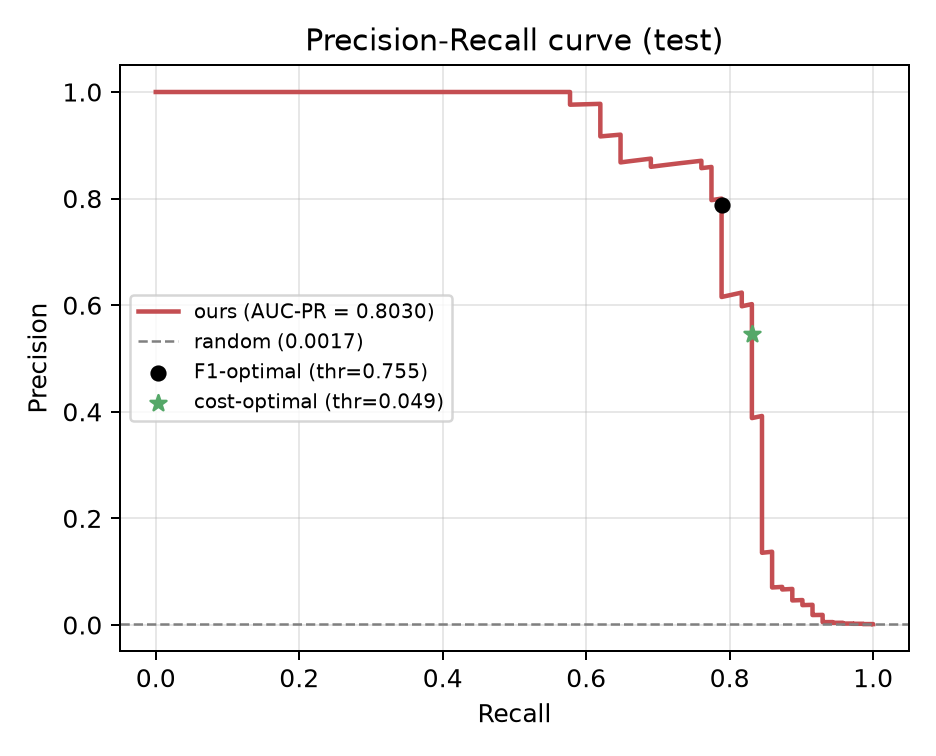
\includegraphics[width=0.92\columnwidth]{fig/pr_curve.png}
  \caption{Precision--recall curve on the test set. The dashed line is the
  random baseline (equal to the fraud prevalence). The dot marks the operating
  point selected on the validation set.}
  \label{fig:pr}
\end{figure}

\subsection{Threshold and Cost Analysis}
Figure~\ref{fig:pr} shows that the model ranks transactions well but that the
choice of operating point matters far more than the choice of architecture.
For the SMOTE model, $\tau=0.5$ yields a cost of 319, the $F_1$-optimal
threshold $\tau_{F1}=0.755$ yields 315, and the cost-optimal threshold
$\tau_{cost}=0.049$ yields 289---an 9.4\% reduction relative to the default
while raising recall from 0.789 to 0.831. The gap is small in absolute terms
because this model is already well calibrated; the same comparison on the
class-weighted model is far more dramatic, where $\tau=0.5$ costs 1192 and
$\tau_{cost}=0.966$ costs 302, a 75\% reduction.

Two lessons follow. First, $F_1$ is the wrong objective when the two error
types have unequal cost: on three of the nine configurations the
$F_1$-optimal threshold is \emph{worse} than doing nothing, i.e.\
$\mathrm{Cost}(\tau_{F1}) > \mathrm{Cost}(0.5)$ (369 vs 289 for random
oversampling, 390 vs 309 for weighted sampling, 332 vs 327 for GBDT). Second,
the cost-optimal threshold recovers the value predicted by \eqref{eq:taustar},
which means the whole calibration problem can be stated in one line: the
default threshold is wrong, and how wrong depends on the cost ratio, not on
the resampling strategy.

\begin{figure}[t]
  \centering
  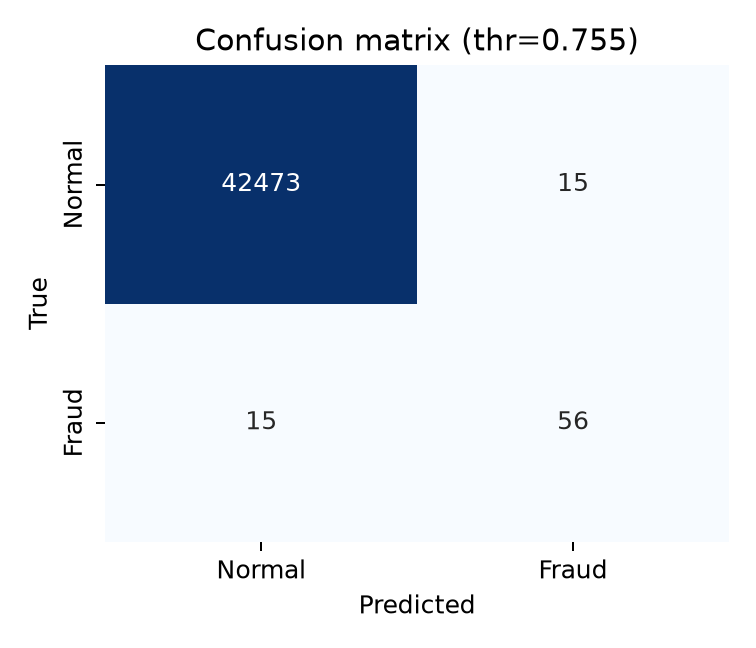
\includegraphics[width=0.9\columnwidth]{fig/confusion_matrix.png}
  \caption{Confusion matrix at the tuned threshold.}
  \label{fig:cm}
\end{figure}

\begin{figure}[t]
  \centering
  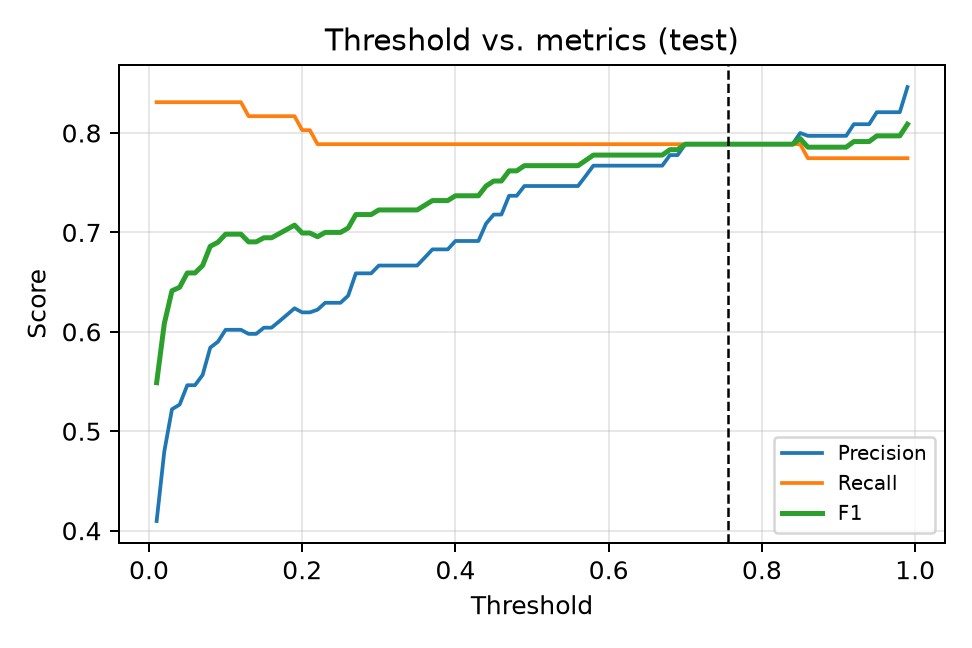
\includegraphics[width=0.92\columnwidth]{fig/threshold_curve.png}
  \caption{Precision, recall and $F_1$ as a function of the threshold. The
  vertical line marks the selected operating point.}
  \label{fig:thr}
\end{figure}

\begin{figure}[t]
  \centering
  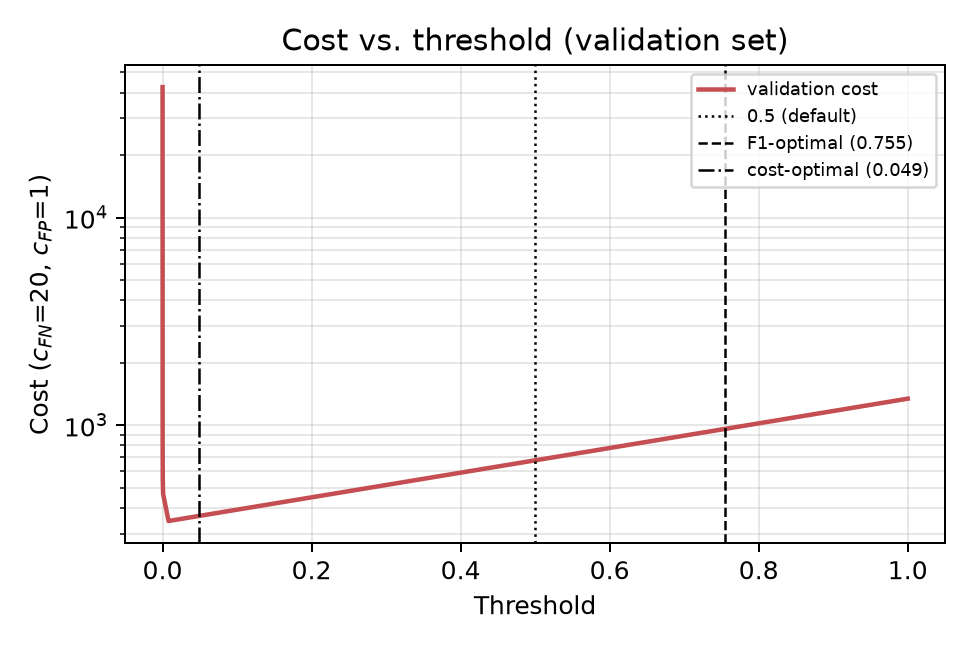
\includegraphics[width=0.92\columnwidth]{fig/cost_curve.png}
  \caption{Business cost against the decision threshold, measured on the
  validation split (the split on which the threshold is selected). The cost is
  flat over a wide range and rises sharply on both sides, which is why a
  threshold must be selected rather than inherited.}
  \label{fig:cost}
\end{figure}

\subsection{Deployment}
The model is served through a Gradio application.
Users upload a CSV of raw transactions; the service scales the inputs with the
stored scaler, scores every row, flags those above the cost-optimal threshold,
and returns the results sorted by risk. Batch scoring costs 0.02~ms per row; a
single row costs about 6~ms once call overhead is included. On a demonstration
file of 2{,}060 transactions containing 60 frauds, the deployed model flags 57
transactions, of which 56 are genuine frauds, i.e.\ it recovers 93\% of the
frauds at one false alarm. The demonstration file deliberately raises the fraud
rate to 2.9\% so that the interface has something to show; at the true
prevalence of 0.17\%, 2{,}000 transactions would contain about three frauds.

% TODO: 打开 python app.py --ckpt runs/mlp_smote/best.pt，上传 data/demo_transactions.csv
%       点"开始检测"后截一张图存成 report/fig/demo.png，再把下面三行的注释符删掉。
% \begin{figure}[t]
%   \centering
%   \includegraphics[width=0.95\columnwidth]{fig/demo.png}
%   \caption{Deployment interface: batch scoring with per-transaction risk and
%   a downloadable result file.}
%   \label{fig:demo}
% \end{figure}

% ---------------------------------------------------------------- IV
\section{Challenges and Conclusion}
\label{sec:conclusion}

\subsection{Challenges Encountered}
\begin{itemize}
  \item \textbf{We were wrong about the baseline.} We expected the unweighted
        model to collapse, and wrote that expectation into our first draft. The
        measured AUC-PR was 0.7196 with a recall of 0.789---within noise of the
        best model. The real defect of that baseline was the default threshold,
        not the learned representation. Correcting this claim changed the
        paper's main message.
  \item \textbf{The 0.5 threshold trap.} Class weighting inflated the cost at
        $\tau=0.5$ from 313 to 1192 without improving AUC-PR. This was the
        first evidence that re-weighting changes the probability scale rather
        than the ranking, and it motivated the closed-form threshold
        \eqref{eq:taustar}.
  \item \textbf{$F_1$ is not a cost.} Selecting the threshold by maximum $F_1$
        made three of nine configurations \emph{worse} than $\tau=0.5$. We had
        initially reported the $F_1$-optimal threshold as ``the tuned
        threshold'' and would have shipped a model that was more expensive than
        the default.
  \item \textbf{Architecture can hurt.} The 1D-CNN, added as an ``advanced''
        model, lost 33 AUC-PR points relative to the plain MLP. Convolution
        assumes that adjacent features are related, which is false for PCA
        components ordered arbitrarily by variance.
\end{itemize}

\subsection{Limitations}
The evaluation uses a single dataset whose test set contains only 71 fraud
cases, so single-number metrics fluctuate by roughly three points and the
eight-point AUC-PR gap between resampling and no handling, while consistent
across three resampling variants, is not accompanied by per-seed error bars;
we report curves rather than a single score and treat the ranking as
indicative rather than established. All differences among the top four
configurations (AUC-PR 0.789--0.803, cost 276--298) are within this noise
band, so the choice of SMOTE over weighted sampling is a tie broken by
interpretability, not by evidence. We do not model concept drift, which is
central in production fraud detection, and we assume a fixed cost ratio
$c_{FN}/c_{FP}=20$ rather than estimating it from business data; because
$\tau^{*}$ depends directly on that ratio, the operating point would move if
the assumption changed.

\subsection{Future Work}
Directions include online learning with drift detection, graph neural networks
over the transaction--merchant graph, and cost-sensitive training that optimises
\eqref{eq:cost} directly instead of tuning the threshold post hoc.

\begin{thebibliography}{00}
\bibitem{imbalance} H. He and E. A. Garcia, ``Learning from imbalanced data,'' \textit{IEEE Trans. Knowl. Data Eng.}, vol. 21, no. 9, pp. 1263--1284, 2009.
\bibitem{smote} N. V. Chawla, K. W. Bowyer, L. O. Hall, and W. P. Kegelmeyer, ``SMOTE: Synthetic minority over-sampling technique,'' \textit{J. Artif. Intell. Res.}, vol. 16, pp. 321--357, 2002.
\bibitem{pr} T. Saito and M. Rehmsmeier, ``The precision-recall plot is more informative than the ROC plot when evaluating binary classifiers on imbalanced datasets,'' \textit{PLoS ONE}, vol. 10, no. 3, e0118432, 2015.
\bibitem{dataset} A. Dal Pozzolo, O. Caelen, R. A. Johnson, and G. Bontempi, ``Calibrating probability with undersampling for unbalanced classification,'' in \textit{Proc. IEEE Symp. Comput. Intell. Data Min.}, 2015, pp. 159--166.
\end{thebibliography}

\end{document}
